\documentclass[notes,compress,serif,professionalfont]{beamer}
\usetheme{boxes} %Boadilla, Berkeley, Dresden, Rochester, Pittsburgh
\useoutertheme{miniframes} %split, shadow, infolines, default
\usepackage{hyperref}
\usepackage{pxfonts}
\usepackage{amsmath}
\usepackage{amssymb}
\usepackage{amsfonts}
\usepackage{enumerate}
\usepackage{xcolor}
\usepackage{multirow}
\usepackage{tikz}
\usepackage{subfigure}
\usepackage{graphicx}
\usepackage{caption,subcaption}
\usepackage{caption}
\usetikzlibrary{arrows,shapes}
\beamertemplateballitem % make bullets and items fancy balls
\useheadtemplate{%
\vbox{%
\vskip1pt%
\beamerline{\insertnavigation{\paperwidth}}%
\vskip-5pt
}
}
%\renewcommand{\frametitle}[1]{\begin{center}\textbf{#1}\end{center}}


% Introduce some notational abbreviations
\def\bmx{{\mathbf x}}
\def\bmX{{\mathbf X}}
\def\bmY{{\mathbf Y}}
\def\bbeta{\boldsymbol{\beta}}

\begin{document}
\title{Predicting Bug Resolution on Eclipse Browser}
\author{Al-sadh Imadh, Hope Mullins, Gualberto Oliveira}
\date{1 August 2024}

\begin{frame}
  \titlepage
\end{frame}


\section{Introduction and Motivation}
\begin{frame}
\frametitle{Summary}
   We explored a dataset on bug tracking for the Eclipse Browser. \pause

\bigskip
   Our goal was to analyze the factors that impacted the likelihood of a bug being fixed. \pause

\bigskip
    We trained 5 types of models and found that Random Forest gave the best AUC (Area Under the Curve) score.
    
\end{frame}

\begin{frame}
\frametitle{ROADMAP OF TALK}
  \begin{enumerate}[<+->]
  \item Problem
  \item Theory
  \item Data
  \item Training, Validation, and Testing
  \item Conclusions
  \end{enumerate}
\end{frame}

\section{Problem}
\begin{frame}{Software Bugs}
         Bugs are a big problem in software and cause programs to behave in ways that are unexpected or not at all. \pause 

        \bigskip
        On average, they are quoted to cost nearly \$60 Billion each year. \pause

        \bigskip
        Assignments to developers who will work on fixing the bug sometimes choose to not fix bugs due to just how labor intensive they will be.
\end{frame}

\begin{frame}{Bug Prediction}
         The Eclipse and Mozilla Defect Tracking Dataset contains a plethora of information about bug reports and how they are updated over time. \cite{LamkanfiMSR13}\pause
         
        \bigskip
        We will use this data to predict the likelihood of a bug report being fixed or not fixed. \pause

        \bigskip
        To do this, we will employ 5 types of models on an altered dataset and compare their results to draw conclusions.
\end{frame}

\section{Theory}

\begin{frame}
\frametitle{LOGIT Regression}
  \begin{enumerate}[<+->]
  \item This model takes linear combination of the factors and transforms it to return a value $p \in [0, 1]$
  \item 0 represents "Won't Fix", 1 represents "Fixed"
  \item Our optimal threshold to label output as 1 was 0.56
  \end{enumerate}
  \vspace{1em}
  \begin{itemize}
  \item Regression equation:
$$ \ln{\left(\frac{p}{1-p}\right)}=\beta_0 + \beta_1 x + ... + \beta_k x_k $$
  \end{itemize}
\end{frame}

\begin{frame}{Lasso Regularization}
    \begin{enumerate}[<+->]
    \item This improves the previous LOGIT model by adding to the loss function $L$ 
    $$L + \lambda \sum_i |\beta_i|$$
    \item Model is encouraged to push (and even set) $\beta_i$'s to 0.
    \end{enumerate}
    \centering
    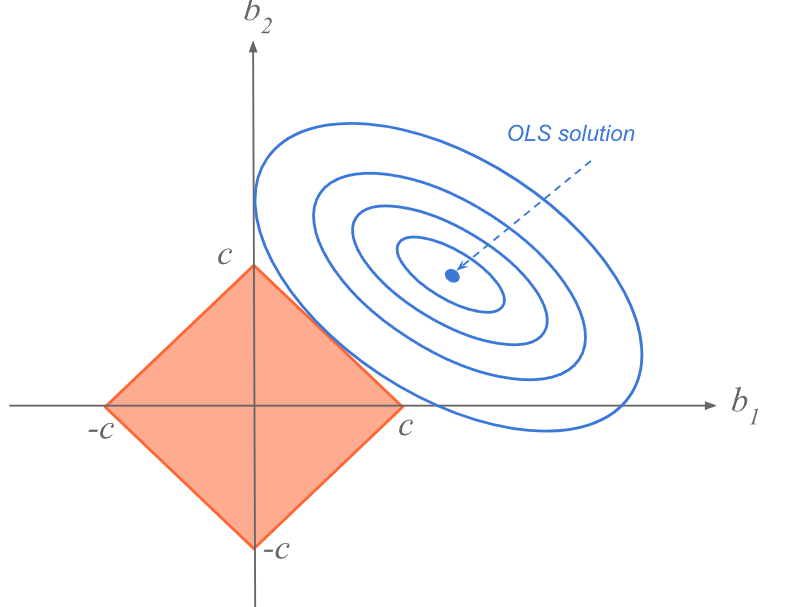
\includegraphics[width=2in]{Lasso.png}
    
    \tiny{https://allmodelsarewrong.github.io/lasso.html}
\end{frame}

\begin{frame}{Bagging}
    Also known as Bootstrap Aggregation.
    \vspace{1em}
    \begin{enumerate}[<+->]
    \item Reduces variance in a noisy dataset
    \item Initial dataset is bootstrapped and each sample is used to make a decision tree
    \item Smaller models are averaged/aggregated to make overall model
    \end{enumerate}
        \centering
    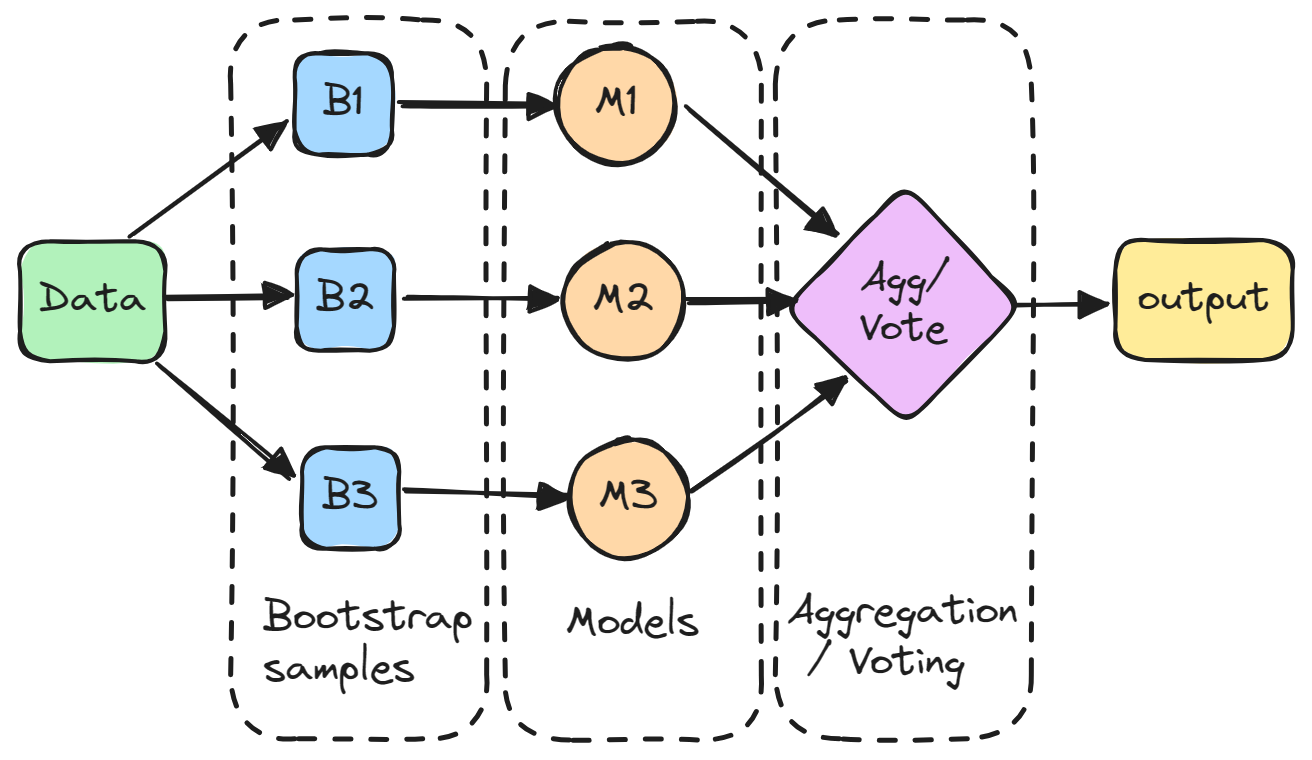
\includegraphics[width=2in]{Bagging.png}
    \tiny{https://www.datacamp.com/tutorial/what-bagging-in-machine-learning-a-guide-with-examples}
    
\end{frame}



\begin{frame}{Random Forest}
    \begin{enumerate}[<+->]
        \item Closely related to Bagging
        \item Unlike bagging, only a handful of the variables are considered during a node split
        \item The variables are chosen randomly during training
        \item The random selection leads to more independent trees which can help prediction
    \end{enumerate}
        \centering
    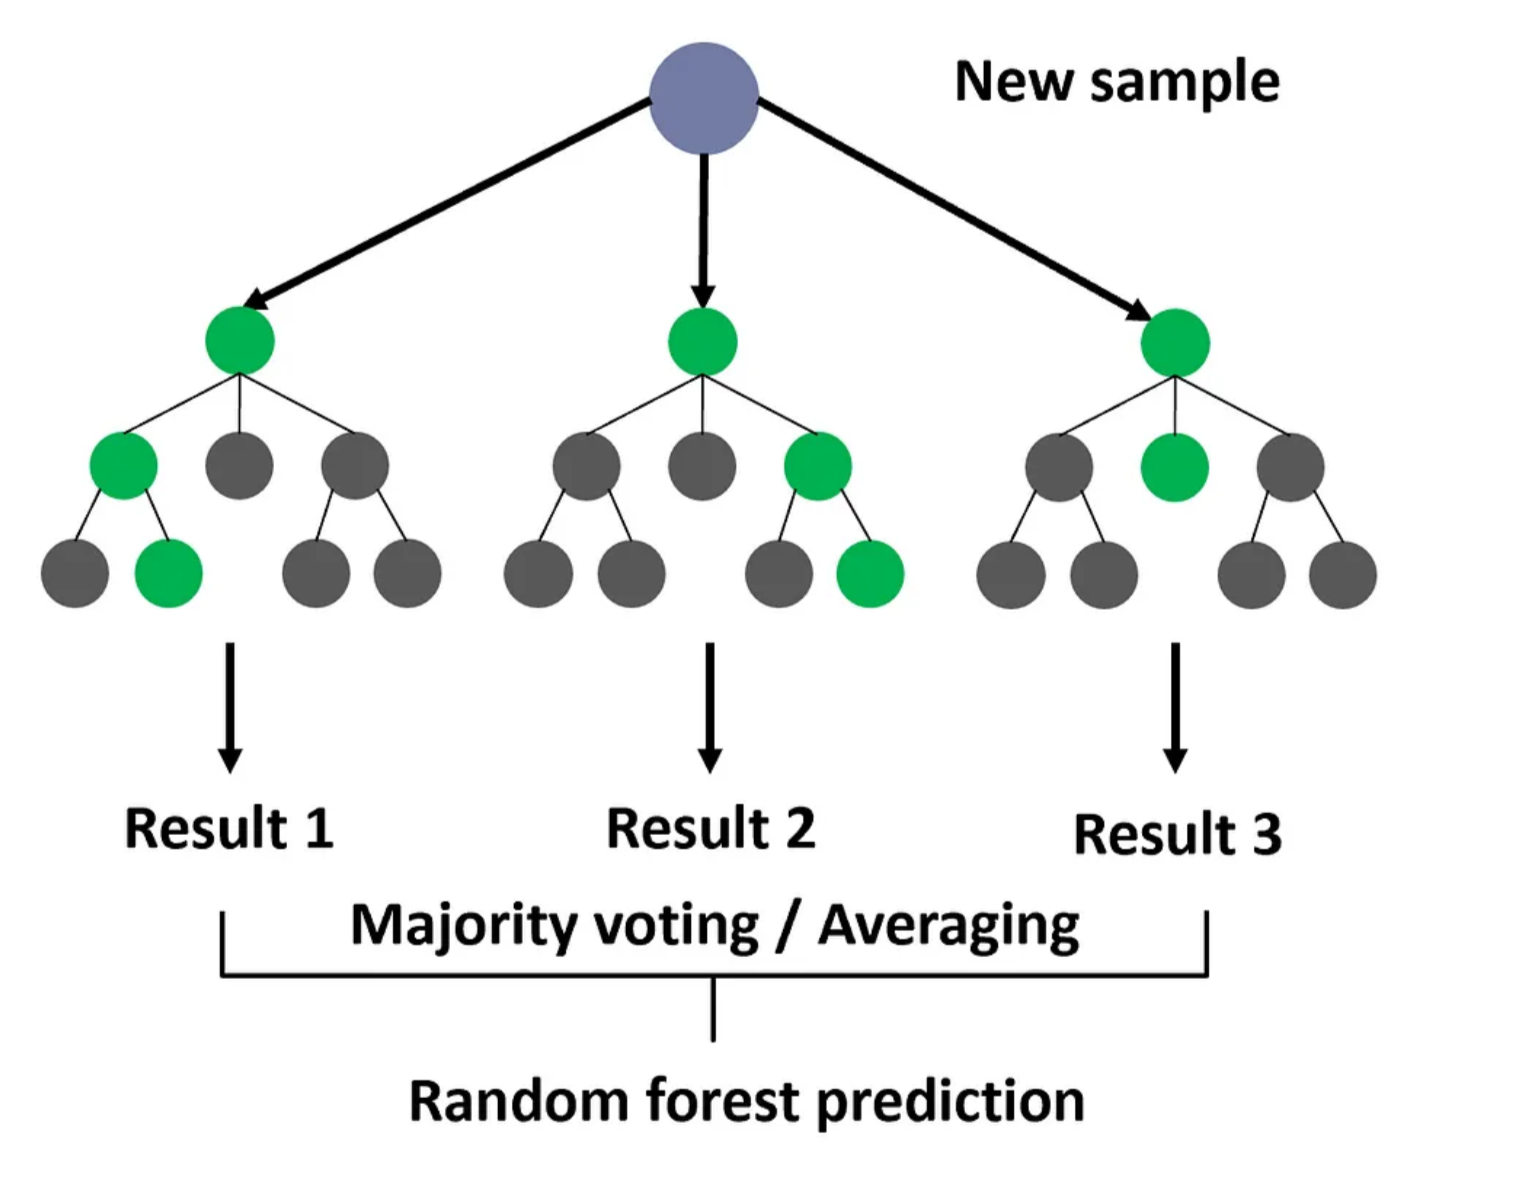
\includegraphics[width=2in]{RForest.png}
    \tiny{https://medium.com/@roiyeho/random-forests-98892261dc49}
\end{frame}

\begin{frame}{Boosting}
    \begin{enumerate}[<+->]
        \item Weak decision trees are built sequentially
        \item Models (Learners) build on top of the previous one, each model weighted on performance
        \item We used Gradient Boosting, which tries to build learners that are more efficient than the previous
    \end{enumerate}
    \centering
    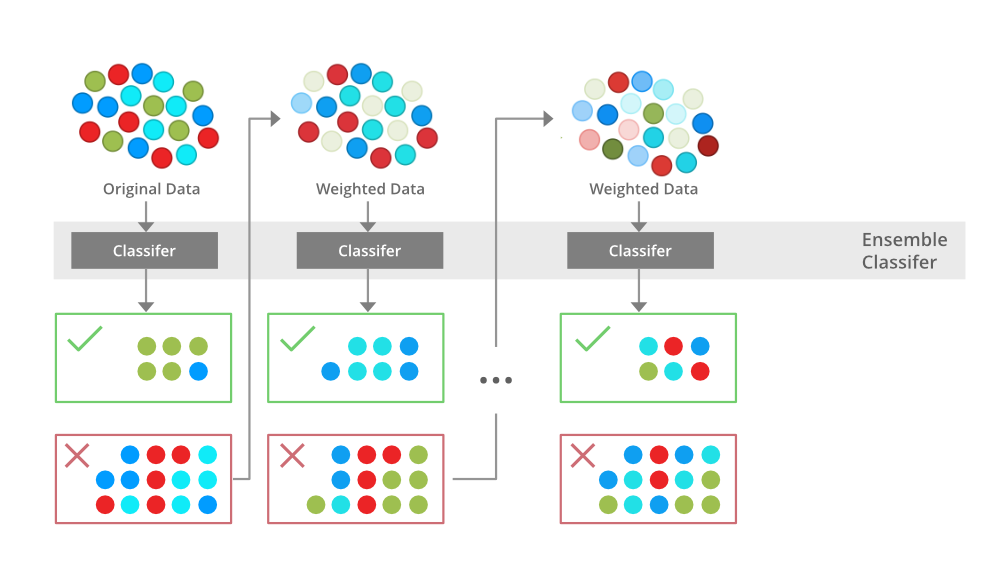
\includegraphics[width=3in]{Boosting.png}
    \tiny{https://www.geeksforgeeks.org/boosting-in-machine-learning-boosting-and-adaboost/}
\end{frame}

\section{Data}
\begin{frame}{Eclipse Bug Tracking Dataset}
    \begin{itemize}
        \item <1- > The Eclipse and Mozilla Defect Tracking Dataset
        \item <2- > 12 Excel files containing attributes about a bug. Attributes are updated over time
        \item <3- > Only bugs labeled "Fixed" or "Won't Fix" are kept. Duplicate bugs removed. Final dataset has size of 90,797
        \item <4- > New variables created using information in dataset
        \item <5- > Excel and SQLite3 were used to cleanup the data and create new variables
    \end{itemize}
\end{frame}

\begin{frame}{Data Structure}
    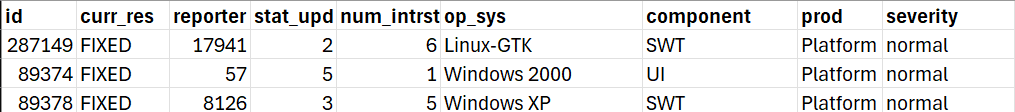
\includegraphics[width=\linewidth]{Sample_data.png}

\bigskip
    Sample of dataset. Some new variables include: \pause
    \begin{itemize}
        \item Total time bug report is open
        \item Max priority/severity
        \item Number of reassignments/status changes
        \item Success rate of initial assignee
    \end{itemize}
\end{frame}

\begin{frame}{Variable Descriptions (1)}
    \begin{itemize}
        \item id: Unique identifier for bug
        \item curr\_res: Whether a bug is fixed or won't be fixed
        \item reporter: Unique identifier for the bug reporter
        \item stat\_upd: Number of times the bug status was updated
        \item num\_intrst: Number of emails interested in the bug
        \item op\_sys: Operating system that bug affects. Most recent update value used
        \item prod: Software/product that the bug pertains to
        \item component: Subsystem of product that the bug affects
        \item severity: Highest severity given to the bug
    \end{itemize}
\end{frame}

\begin{frame}{Variable Description (2)}
    \begin{itemize}
        \item version: The version of the product that the bug affects
        \item times\_assigned: Number of times the bug was reassigned
        \item succ\_rate: The success rate of the initial assignee
        \item res\_upd: Number of times the resolution of a bug was changed
        \item res\_time: Time until the bug was resolved
        \item reporter\_report\_cnt: How many bugs the reporter has reported in the dataset
        \item desc\_length: Sum of lengths of the descriptions on the bug
        \item prio: Highest priority value assigned to the bug
    \end{itemize}
\end{frame}

\section{Models}

\begin{frame}{Model: LOGIT Regression (with poly)}
    \begin{figure}
        \centering
        \begin{minipage}{.5\textwidth}
            \centering
            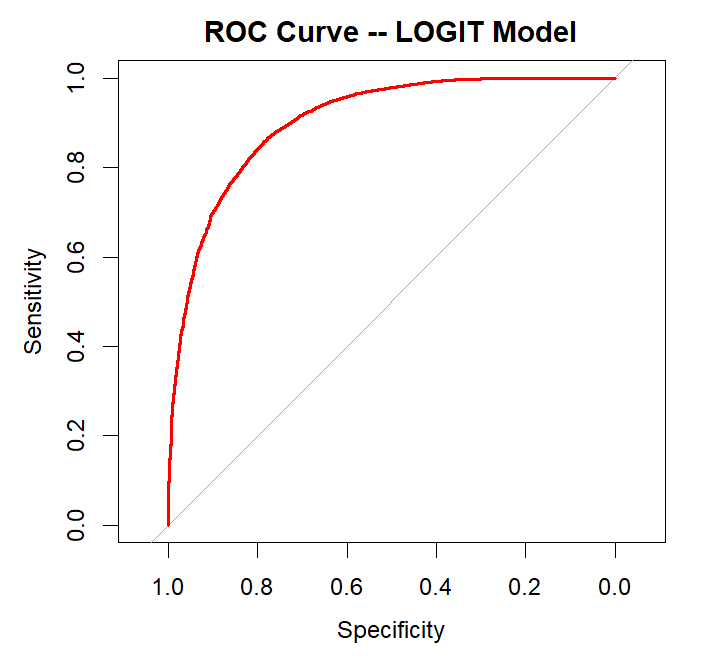
\includegraphics[width=\linewidth]{Logit ROC.png}
        \end{minipage}%
        \begin{minipage}{.5\textwidth}
            \caption*{Confusion Matrix}
            \begin{table}
            \centering
            \resizebox{5cm}{!}{%
            \begin{tabular}{||l|c|c||}
                \hline
                 class & Wont Fix & Fixed \\
                 \hline
                 Wont Fix & 2848 & 777\\
                 Fixed & 3070 & 29624 \\
                 \hline
            \end{tabular}
            }% 
            \end{table}
        \end{minipage}
    \caption{AUC: 0.9048}
    \end{figure}
\end{frame}

\begin{frame}{Model: LASSO Regularization (with poly)}
    \begin{figure}
        \centering
        \begin{minipage}{.5\textwidth}
            \centering
            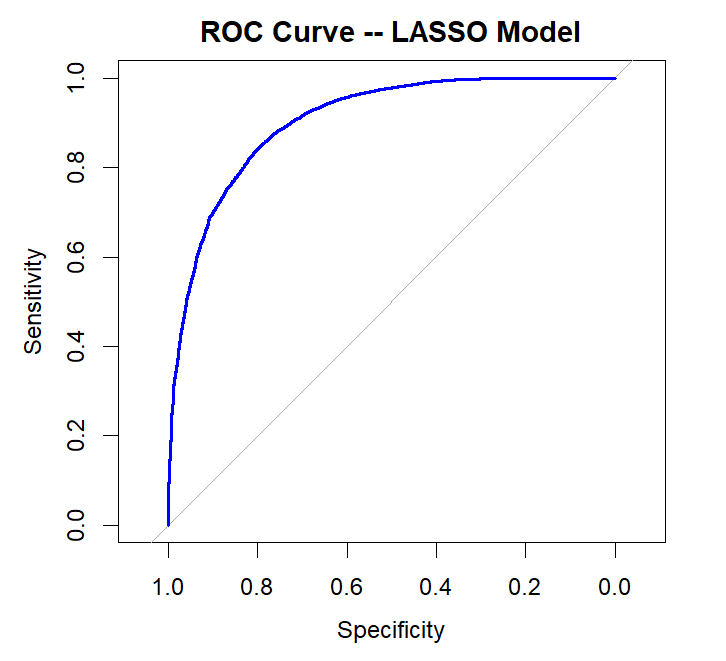
\includegraphics[width=\linewidth]{LASSO ROC.png}
        \end{minipage}%
        \begin{minipage}{.5\textwidth}
            \caption*{Confusion Matrix}
            \begin{table}
            \centering
            \resizebox{5cm}{!}{%
            \begin{tabular}{||l|c|c||}
                \hline
                 class & Wont Fix & Fixed \\
                 \hline
                 Wont Fix & 3161 & 826\\
                 Fixed & 2757 & 29575 \\
                 \hline
            \end{tabular}
            }% 
            \end{table}
        \end{minipage}
    \caption{AUC: 0.9286}
    \end{figure}
\end{frame}

\begin{frame}{Model: Bagging}
    \begin{figure}
        \centering
        \begin{minipage}{.5\textwidth}
            \centering
            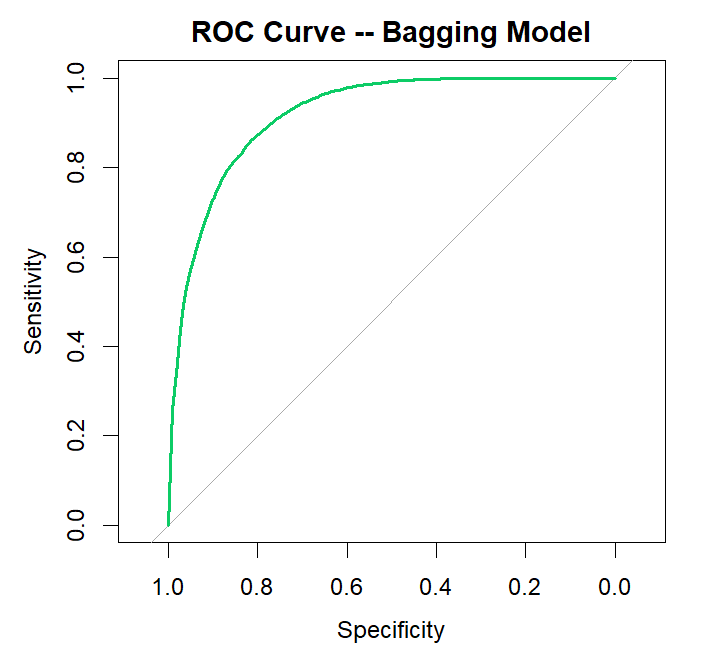
\includegraphics[width=\linewidth]{Bagging ROC.png}
        \end{minipage}%
        \begin{minipage}{.5\textwidth}
            \caption*{Confusion Matrix}
            \begin{table}
            \centering
            \resizebox{5cm}{!}{%
            \begin{tabular}{||l|c|c||}
                \hline
                 class & Wont Fix & Fixed \\
                 \hline
                 Wont Fix & 3425 & 521\\
                 Fixed & 2493 & 29880 \\
                 \hline
            \end{tabular}
            }% 
            \end{table}
        \end{minipage}
    \caption{AUC: 0.9186}
    \end{figure}
\end{frame}

\begin{frame}{Model: Random Forest}
    \begin{figure}
        \centering
        \begin{minipage}{.5\textwidth}
            \centering
            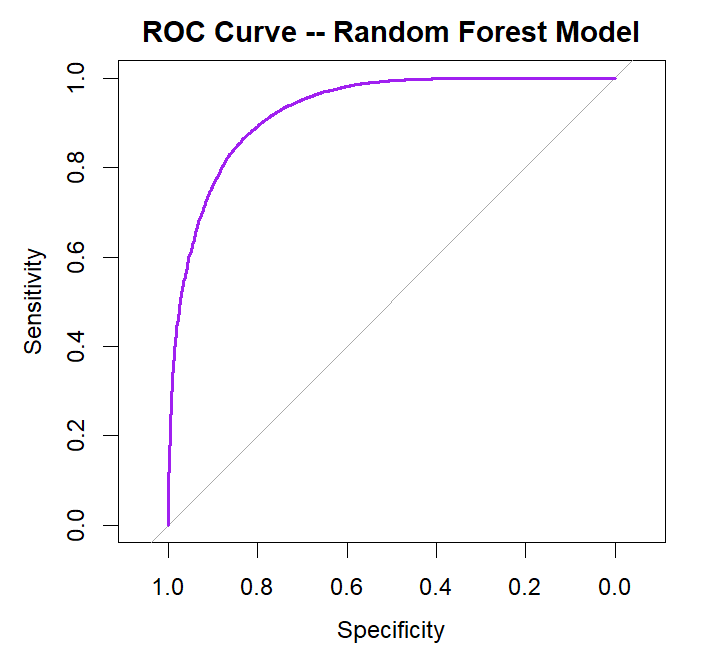
\includegraphics[width=0.8\linewidth]{RF ROC.png}
        \end{minipage}%
        \begin{minipage}{.5\textwidth}
            \caption*{Confusion Matrix}
            \begin{table}
            \centering
            \resizebox{5cm}{!}{%
            \begin{tabular}{||l|c|c||}
                \hline
                 class & Wont Fix & Fixed \\
                 \hline
                 Wont Fix & 3431 & 438\\
                 Fixed & 2487 & 29963 \\
                 \hline
            \end{tabular}
            }% 
            \end{table}
        \end{minipage}
    \caption{AUC: 0.9286}
    \end{figure}    
\end{frame}

\begin{frame}{Model: Boosting}
    \begin{figure}
        \centering
        \begin{minipage}{.5\textwidth}
            \centering
            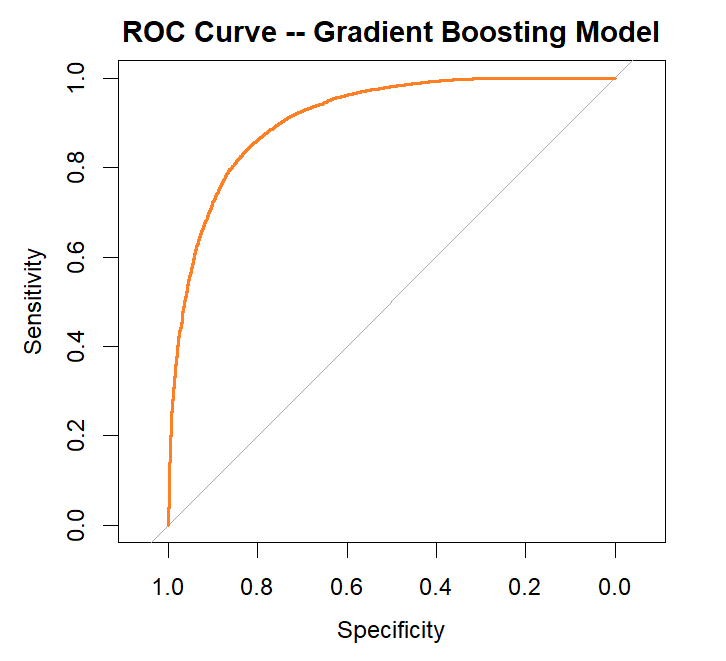
\includegraphics[width=0.8\linewidth]{Boosting ROC.png}
        \end{minipage}%
        \begin{minipage}{.5\textwidth}
            \caption*{Confusion Matrix}
            \begin{table}
            \centering
            \resizebox{5cm}{!}{%
            \begin{tabular}{||l|c|c||}
                \hline
                 class & Wont Fix & Fixed \\
                 \hline
                 Wont Fix & 3349 & 916\\
                 Fixed & 2569 & 29485 \\
                 \hline
            \end{tabular}
            }% 
            \end{table}
        \end{minipage}
    \caption{AUC: 0.9122}
    \end{figure}
    
\end{frame}

\section{Conclusion}

\begin{frame}{Important Variables}
    \begin{enumerate}[<+->]
        \item Based on the results of the LOGIT regression and the subsequent LASSO regularization
        \item Almost every variable we examined was significant
        \item The only variable that was found to not be significant was "Component"
    \end{enumerate}
\end{frame}

\begin{frame}{Summary of LOGIT variables (no poly)}
    \begin{table}[ht]
    \centering
    \resizebox{9cm}{!}{%
    \begin{tabular}{r|r|r|r|r}
    \hline
     & Estimate & Std. Error & z value & Pr($>$$|$z$|$) \\ 
      \hline
    (Intercept) & -2.4051 & 0.1819 & -13.22 & 0.0000 \\ 
      reporter & -0.0000 & 0.0000 & -19.40 & 0.0000 \\ 
      stat\_upd & 0.5816 & 0.0208 & 27.90 & 0.0000 \\ 
      num\_intrst & 0.1420 & 0.0095 & 14.99 & 0.0000 \\ 
      op\_sys & 0.0039 & 0.0012 & 3.25 & 0.0012 \\ 
      component & -0.0007 & 0.0016 & -0.40 & 0.6888 \\ 
      prod & -0.1186 & 0.0179 & -6.62 & 0.0000 \\ 
      severity & 0.2028 & 0.0113 & 17.90 & 0.0000 \\ 
      version & 0.0382 & 0.0025 & 15.53 & 0.0000 \\ 
      times\_assigned & 0.2017 & 0.0179 & 11.28 & 0.0000 \\ 
      succ\_rate & 5.1959 & 0.1233 & 42.15 & 0.0000 \\ 
      res\_upd & -0.7482 & 0.0322 & -23.26 & 0.0000 \\ 
      res\_time & -0.0000 & 0.0000 & -46.34 & 0.0000 \\ 
      reporter\_report\_cnt & -0.0002 & 0.0000 & -15.26 & 0.0000 \\ 
      desc\_length & -0.0022 & 0.0003 & -6.46 & 0.0000 \\ 
      prio & -0.1457 & 0.0151 & -9.65 & 0.0000 \\ 
       \hline
    \end{tabular}
    }%
    \end{table}
\end{frame}

\begin{frame}{ROC Curve Comparison}
    \centering
    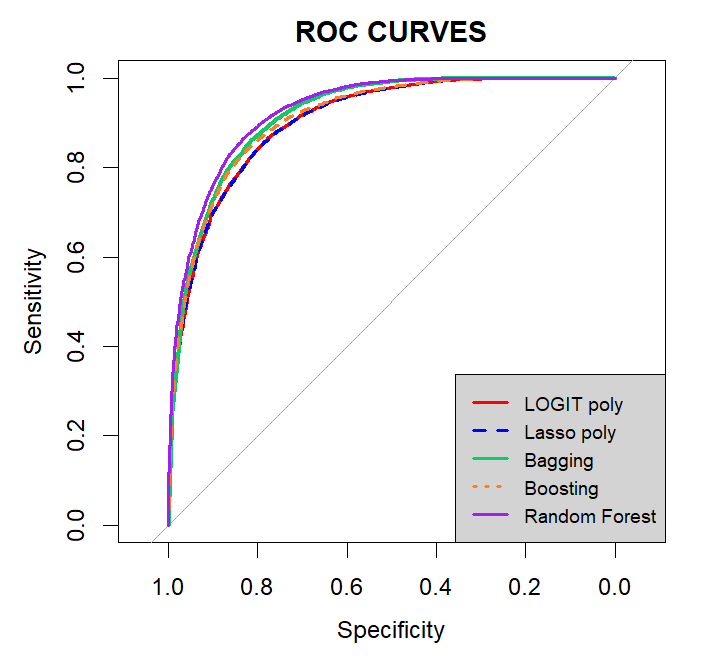
\includegraphics[width=0.75\linewidth]{ROC.png}
\end{frame}


\begin{frame}{Selection of Best Model}
    \begin{enumerate}[<+->]
        \item All models but bagging were also tested using poly() to give 135 variables (including polynomial combinations and interaction effects), with LOGIT and LASSO seeing the most notable improvements
        \item Boosting also improved, but not enough to outperform our Random Forest model
        \item We used the Area Under the Curve to determine our best model. Without poly(), Boosting, Random Forest, and Bagging all returned similarly high AUC scores
        \item Using our training/testing set, Random Forest gave the highest AUC, i.e. the best testing performance, regardless of whether we utilized the poly() function or not.
    \end{enumerate}
\end{frame}

\begin{frame}{Final Notes}
    \begin{enumerate}[<+->]
        \item Each model was a good predictor of how a bug would be resolved
        \item The confusion matrix shows that every model struggles to identify when a bug will not be fixed correctly (considering that the majority of the data consisted of "FIXED" bugs, this makes sense)
        \item In line with the AUC scores, Random Forest identifies both categories the best with Bagging at a close second
        \item Boosting was expected to outperform every other model but ranked below both Bagging and Random Forest
        \item Rankings could change with different val/train splits
    \end{enumerate}
\end{frame}

\begin{frame}{Citation}
    \bibliographystyle{amsalpha}
    \bibliography{Sources.bib}
\end{frame}
        
\end{document}
